\let\negmedspace\undefined
\let\negthickspace\undefined
\documentclass[journal,12pt,twocolumn]{IEEEtran}
%\documentclass[conference]{IEEEtran}
%\IEEEoverridecommandlockouts
% The preceding line is only needed to identify funding in the first footnote. If that is unneeded, please comment it out.
\usepackage{cite}
\usepackage{amsmath,amssymb,amsfonts,amsthm}
\usepackage{algorithmic}
\usepackage{graphicx}
\usepackage{textcomp}
\usepackage{xcolor}
\usepackage{txfonts}
\usepackage{listings}
\usepackage{enumitem}
\usepackage{mathtools}
\usepackage{gensymb}
\usepackage[breaklinks=true]{hyperref}
\usepackage{tkz-euclide} % loads  TikZ and tkz-base
\usepackage{listings}
\DeclareMathOperator*{\Res}{Res}
%\renewcommand{\baselinestretch}{2}
\renewcommand\thesection{\arabic{section}}
\renewcommand\thesubsection{\thesection.\arabic{subsection}}
\renewcommand\thesubsubsection{\thesubsection.\arabic{subsubsection}}

\renewcommand\thesectiondis{\arabic{section}}
\renewcommand\thesubsectiondis{\thesectiondis.\arabic{subsection}}
\renewcommand\thesubsubsectiondis{\thesubsectiondis.\arabic{subsubsection}}

% correct bad hyphenation here
\hyphenation{op-tical net-works semi-conduc-tor}
\def\inputGnumericTable{}                                 %%

\lstset{
	%language=C,
	frame=single, 
	breaklines=true,
	columns=fullflexible
}
\newcommand{\define}{\stackrel{\triangle}{=}}
\newcommand{\permcomb}[4][0mu]{{{}^{#3}\mkern#1#2_{#4}}}
\newcommand{\comb}[1][-1mu]{\permcomb[#1]{C}}

\begin{document}
	%
	
	
	\newtheorem{theorem}{Theorem}[section]
	\newtheorem{problem}{Problem}
	\newtheorem{proposition}{Proposition}[section]
	\newtheorem{lemma}{Lemma}[section]
	\newtheorem{corollary}[theorem]{Corollary}
	\newtheorem{example}{Example}[section]
	\newtheorem{definition}[problem]{Definition}
	%\newtheorem{thm}{Theorem}[section] 
	%\newtheorem{defn}[thm]{Definition}
	%\newtheorem{algorithm}{Algorithm}[section]
	%\newtheorem{cor}{Corollary}
	\newcommand{\BEQA}{\begin{eqnarray}}
		\newcommand{\EEQA}{\end{eqnarray}}
	%	\newcommand{\define}{\stackrel{\triangle}{=}}
	
	\bibliographystyle{IEEEtran}
	%\bibliographystyle{ieeetr}
	
	
	\providecommand{\mbf}{\mathbf}
	\providecommand{\pr}[1]{\ensuremath{\Pr\left(#1\right)}}
	\providecommand{\qfunc}[1]{\ensuremath{Q\left(#1\right)}}
	\providecommand{\sbrak}[1]{\ensuremath{{}\left[#1\right]}}
	\providecommand{\lsbrak}[1]{\ensuremath{{}\left[#1\right.}}
	\providecommand{\rsbrak}[1]{\ensuremath{{}\left.#1\right]}}
	\providecommand{\brak}[1]{\ensuremath{\left(#1\right)}}
	\providecommand{\lbrak}[1]{\ensuremath{\left(#1\right.}}
	\providecommand{\rbrak}[1]{\ensuremath{\left.#1\right)}}
	\providecommand{\cbrak}[1]{\ensuremath{\left\{#1\right\}}}
	\providecommand{\lcbrak}[1]{\ensuremath{\left\{#1\right.}}
	\providecommand{\rcbrak}[1]{\ensuremath{\left.#1\right\}}}
	\theoremstyle{remark}
	\newtheorem{rem}{Remark}
	\newcommand{\sgn}{\mathop{\mathrm{sgn}}}
	\providecommand{\abs}[1]{\left\vert#1\right\vert}
	\providecommand{\res}[1]{\Res\displaylimits_{#1}} 
	\providecommand{\norm}[1]{\left\lVert#1\right\rVert}
	%\providecommand{\norm}[1]{\lVert#1\rVert}
	\providecommand{\mtx}[1]{\mathbf{#1}}
	\providecommand{\mean}[1]{E\left[ #1 \right]}
	\providecommand{\fourier}{\overset{\mathcal{F}}{ \rightleftharpoons}}
	%\providecommand{\hilbert}{\overset{\mathcal{H}}{ \rightleftharpoons}}
	\providecommand{\system}{\overset{\mathcal{H}}{ \longleftrightarrow}}
	%\newcommand{\solution}[2]{\textbf{Solution:}{#1}}
	\newcommand{\solution}{\noindent \textbf{Solution: }}
	\newcommand{\cosec}{\,\text{cosec}\,}
	\providecommand{\dec}[2]{\ensuremath{\overset{#1}{\underset{#2}{\gtrless}}}}
	\newcommand{\myvec}[1]{\ensuremath{\begin{pmatrix}#1\end{pmatrix}}}
	\newcommand{\mydet}[1]{\ensuremath{\begin{vmatrix}#1\end{vmatrix}}}		
		\vspace{3cm}
		
		\title{
			%	\logo{
				Hardware Project - AI1110
				%	}
		}
		\author{Mayank Parasramka\\
			AI22BTECH11018
		}	
		
\maketitle

\newpage
\bigskip
\renewcommand{\thefigure}{\theenumi}
\renewcommand{\thetable}{\theenumi}
\textbf{Description:-} \raggedright\\
\textbf{In my assignment I've made a Random number generator using decoder, flip flops, XOR gate, 555IC}
\tableofcontents
\section{Components used}
\begin{enumerate}[label=(\roman*)]
\item Breadboard
\item Seven Segment Display - Common Anode
\item 7447 Seven Segment Display Decoder
\item 7474 D FlipFlop x2
\item 7486 XOR gate
\item 555 precision timer
\item Resistor 10MΩ
\item Resistor 1KΩ
\item Capacitor 47nF
\item Capacitor 470nF
\item USB micro B breakout board
\item Jumper wires
\end{enumerate}
\section{Setup}
\begin{enumerate}
\item This circuit uses 5V from microusb.
\item This acts as the Vcc of the circuit.
\item The buses are at Vcc, Ground and Clock.
\end{enumerate}
\section{Description}
\begin{enumerate}
	\item The random number generator circuit is designed to generate random numbers using shift registers, providing a versatile and reliable solution for applications that require randomness. The circuit incorporates various components, including a breadboard, seven-segment display, decoder, flip-flops, XOR gate, 555 timer IC, resistors, capacitors, and jumper wires.
	\begin{figure}[h]
		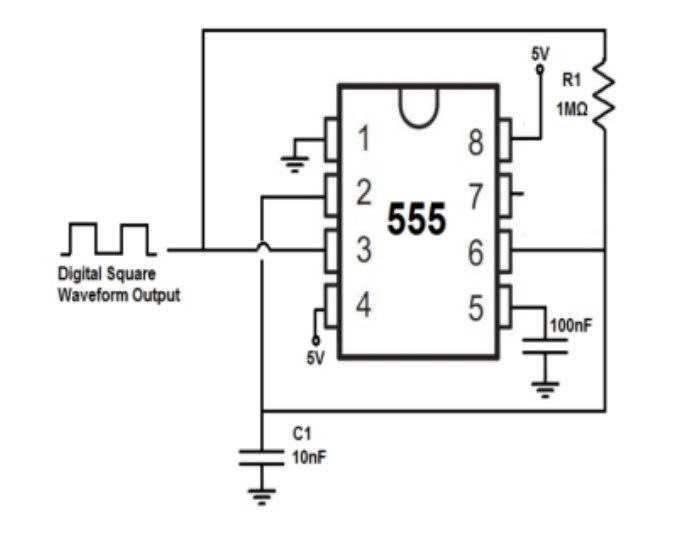
\includegraphics[width=\linewidth]{images/fig07.jpg}
		\caption{Connection in 555 timer circuit}
		\label{555_t_c}
	\end{figure}
	
	\item At the core of the circuit is the shift register, constructed using two D flip-flops (7474 ICs) and an XOR gate (7486 IC). The shift register operates based on the clock signal generated by the 555 timer IC. The clock signal serves as the synchronization mechanism, ensuring the precise shifting of data within the shift register.
	
	\item The clock signal generated by the 555 timer circuit is connected to the CLOCK input of the D flip-flops, enabling the sequential shifting of data through the flip-flops. This shifting action creates a cascading effect, allowing the circuit to generate a sequence of random bits.
	\begin{figure}[h]
		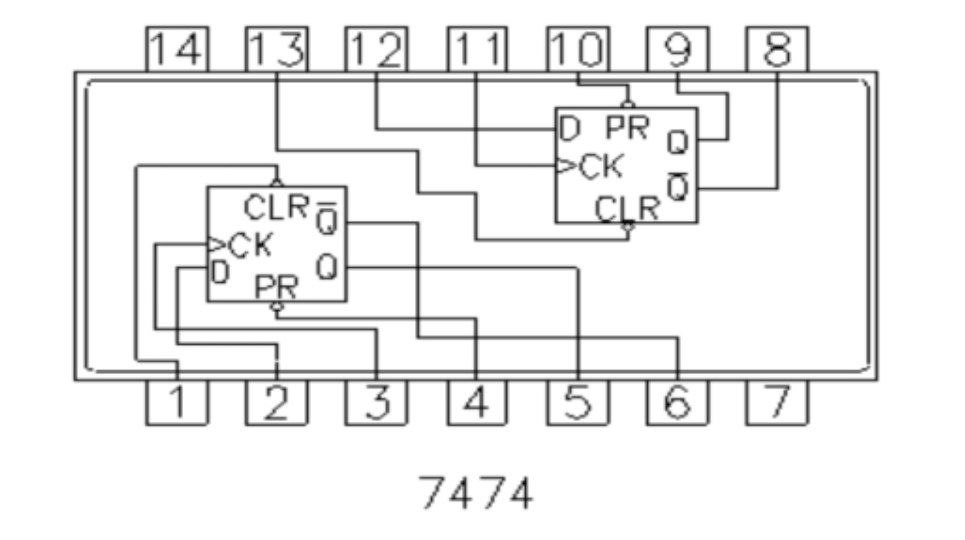
\includegraphics[width=\linewidth]{images/fig03.jpg}
		\caption{Connection in 7474 IC}
		\label{7474_IC}
	\end{figure}

	\item The output of each D flip-flop is connected to the Decoder IC (7447 IC), which converts the binary input into a corresponding output that can be displayed on the seven-segment display. The connections between the flip-flops and the decoder are carefully established to ensure the proper mapping of binary values to the display segments.
	\begin{figure}[h]
		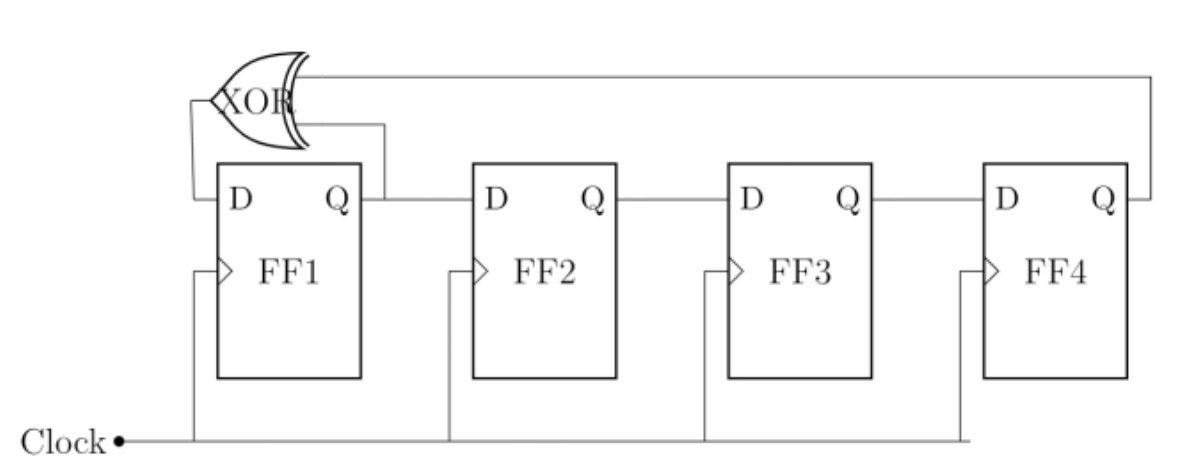
\includegraphics[width=\linewidth]{images/fig04.jpg}
		\caption{Connection in XOR gate}
		\label{XOR}
	\end{figure}
	\begin{figure}[h]
		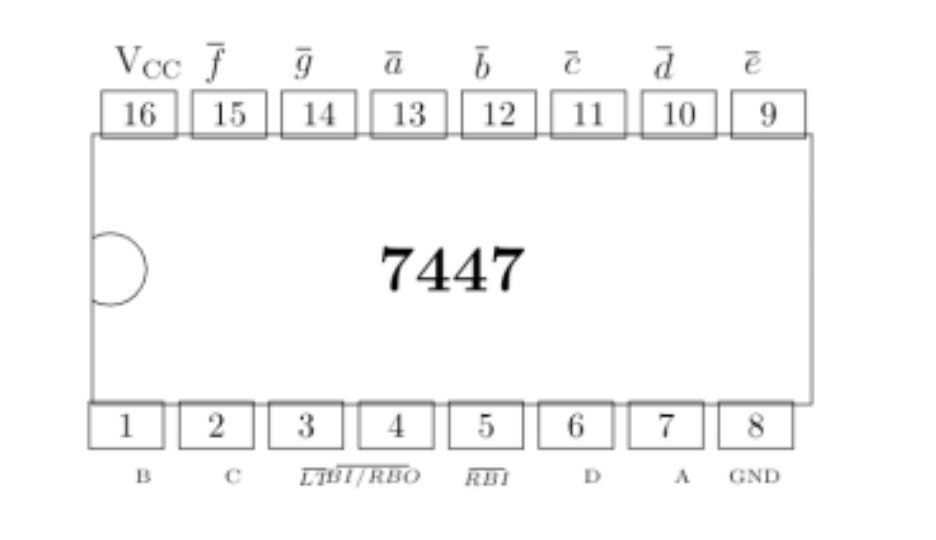
\includegraphics[width=\linewidth]{images/fig01.jpg}
		\caption{Connection in Decoder gate}
		\label{7447}
	\end{figure}
		
	\item The seven-segment display, a common anode type, is connected to the Decoder IC (7447 IC) following the prescribed pin connections. This display arrangement allows the generated random numbers to be visually represented in a human-readable format. Refer to the table \ref{table} and the figure \ref{SSD}.
	\begin{figure}[h]
		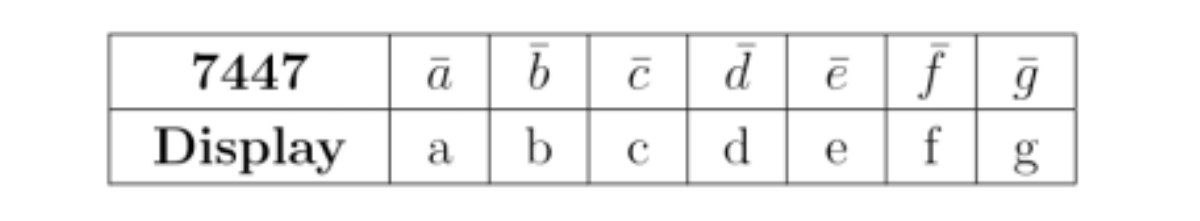
\includegraphics[width=\linewidth]{images/fig02.jpg}
		\caption{Connection of seven segmented display with decoder}
		\label{table}
	\end{figure}
	\begin{figure}[h]
		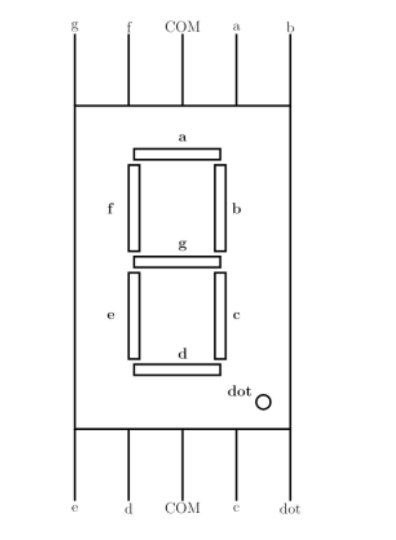
\includegraphics[width=\linewidth]{images/fig05.jpg}
		\caption{Seven segmented display}
		\label{SSD}
	\end{figure}

	\item Power and ground connections are established for all components to ensure proper operation and signal integrity. The circuit requires a stable power supply, and the voltage specifications of each component should be respected to prevent damage and ensure accurate performance.
\section{Applications}
The random number generator circuit using shift registers has several potential applications. Here are some common uses of such a circuit:
\begin{enumerate}
\item Simulations: In computer simulations, random numbers are often required to introduce randomness and variability into the simulated environment. The circuit can be used to generate random numbers that accurately reflect real-world scenarios, enhancing the realism and accuracy of the simulation.

\item Gaming: Randomness is a crucial element in many games, such as dice rolls, card shuffling, or determining the outcome of events. The random number generator circuit can provide a reliable source of random numbers for gaming applications, ensuring fairness and unpredictability.

\item Cryptography: Random numbers play a vital role in cryptographic systems. Randomness is needed for generating cryptographic keys, initialization vectors, and nonces. The circuit can be used to produce high-quality random numbers required for secure communication and encryption protocols.

\item Testing and Quality Assurance: Randomness is often necessary for testing purposes, such as stress testing, software validation, and quality assurance. The circuit can generate random inputs or simulate random events to thoroughly test the functionality, performance, and robustness of systems or software.

\item Decision-Making and Randomized Algorithms: Randomness is employed in decision-making processes and randomized algorithms to introduce uncertainty and avoid biases. The circuit can supply the necessary random numbers to ensure unbiased decision-making or enable the execution of randomized algorithms.
\end{enumerate}
\section{Output} 
	The circuit generates random numbers on the seven segment display. The output is shown in figure \ref{final}
	\begin{figure}[h]
		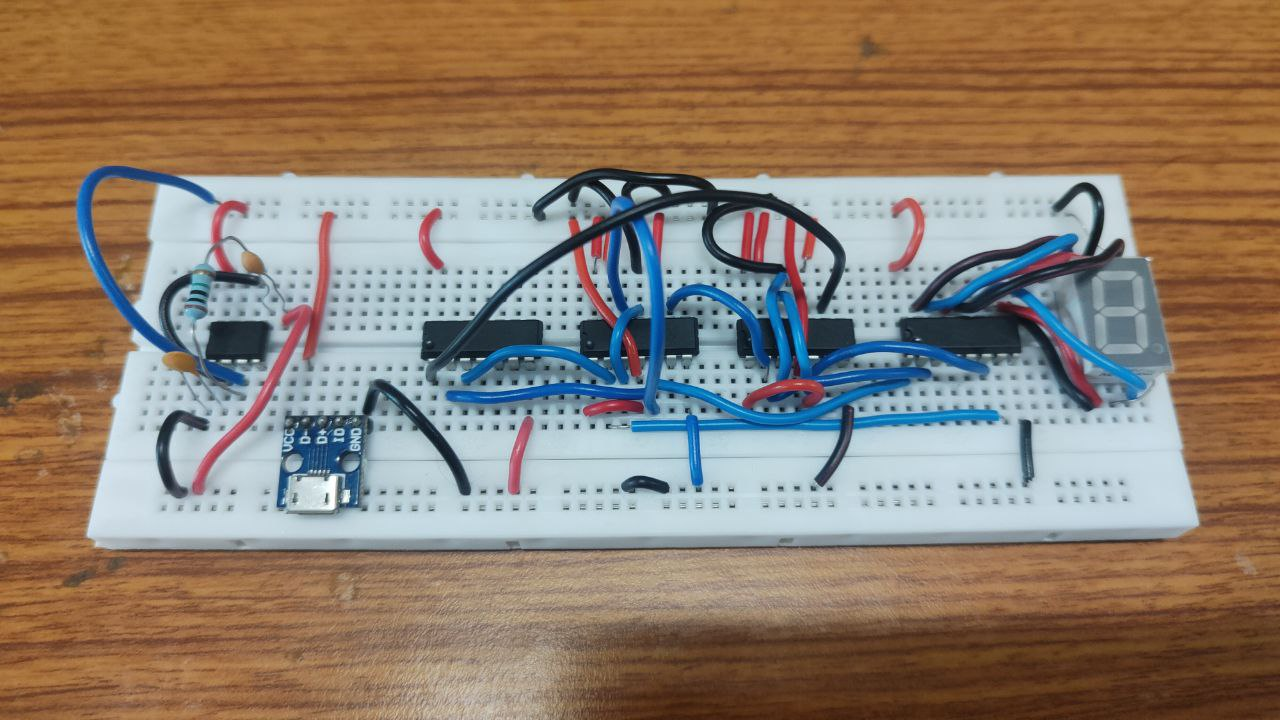
\includegraphics[width = \linewidth]{images/pic1.jpg}
		\caption{output}
		\label{final}
	\end{figure} 
	\begin{figure}[h]
		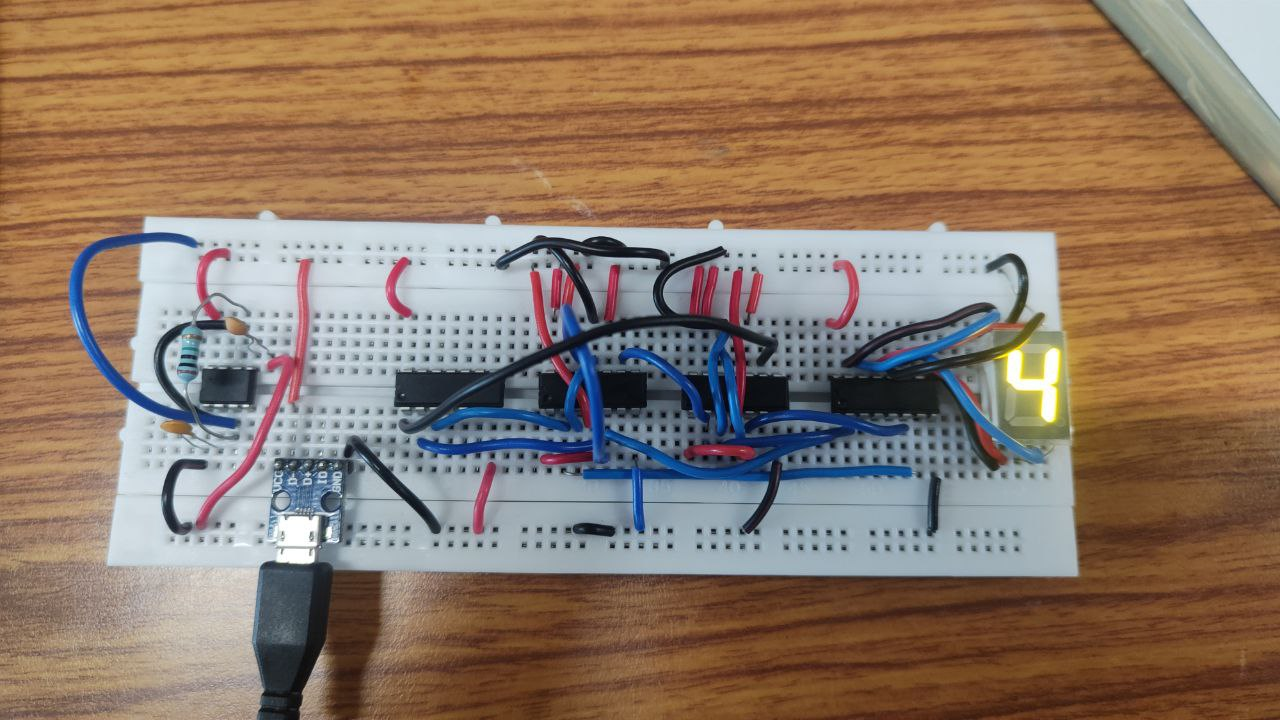
\includegraphics[width = \linewidth]{images/pic2.jpg}
		\caption{output}
		\label{final}
	\end{figure} 
\newpage
\section{Block Diagram}
\begin{figure}[h]
		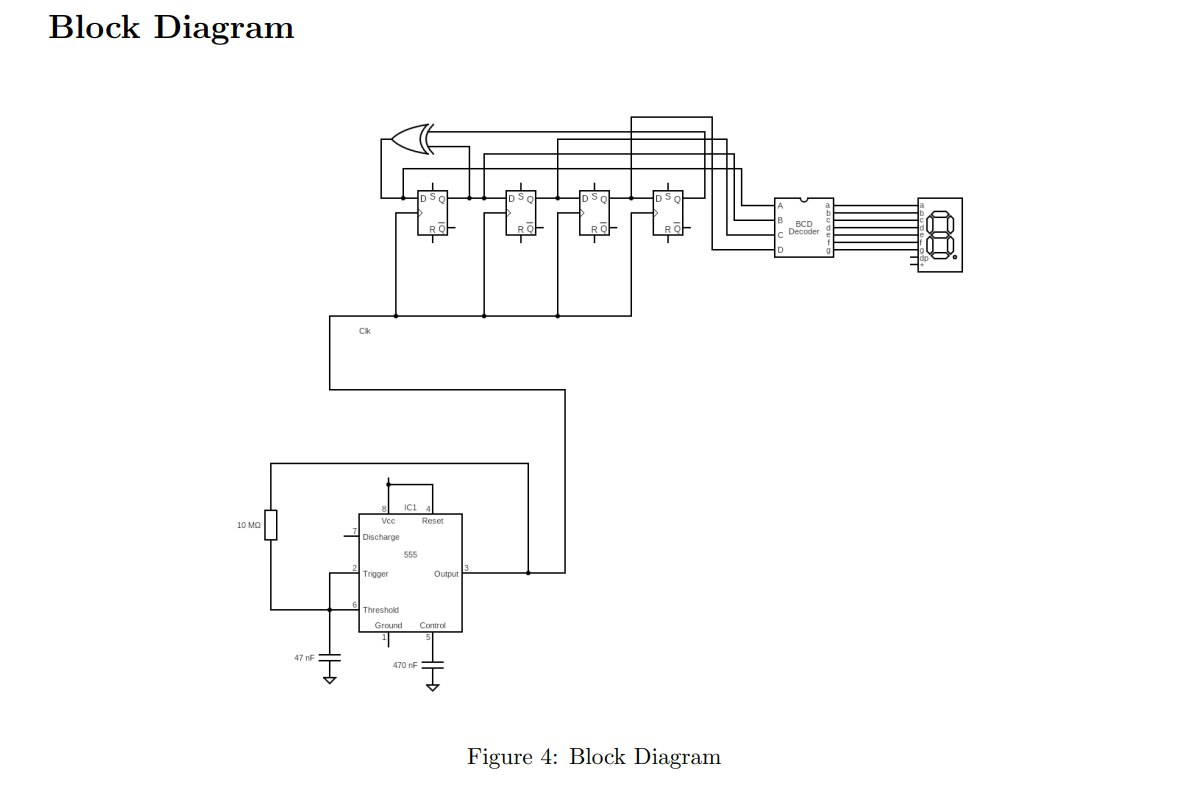
\includegraphics[width= \linewidth]{images/fig06.jpg}
		\caption{Block Diagram}
		\label{SSD}
	\end{figure}
	
\end{enumerate}
\end{document}